% !TeX spellcheck = ru_RU
\documentclass{beamer}
\setbeamertemplate{navigation symbols}{}


\usetheme{Frankfurt}

\usepackage{amsmath,amssymb,amsthm,amscd,amsfonts, mathtools}
\usepackage[utf8]{inputenc}
\usepackage[english, russian]{babel}
\usepackage{wrapfig}
\usepackage{multirow}

\makeatletter
\newcommand*{\rom}[1]{\expandafter\@slowromancap\romannumeral #1@}
\newcommand\setItemnumber[1]{\setcounter{enum\romannumeral\@enumdepth}{\numexpr#1-1\relax}}
\makeatother

\newtheorem{definition_}{Определение}
\newtheorem{target_}{Цель работы}
\newtheorem{prob_task}{Вероятностная постановка задачи классификации}
\newtheorem{algo_task}{Алгоритмическая постановка задачи классификации}
\newtheorem{prob_def}{Вероятностное определение $w_{ij}^k$}
\newtheorem{algo_def}{Алгоритмическое определение $w_{ij}^k$}

\begin{document}
	\title{Синолитические сети в классификации мозговой активности}  
	\author{Власенко Даниил\\
%		\author{Власенко Даниил Владимирович\\
	{\footnotesize Научные руководители: Заикин Алесей, Захаров Денис}
%	{\footnotesize Научные руководитель: Шпилёв Пётр Валерьевич}
	}
	\date{\today} 
	
	\begin{frame}
		\titlepage
	\end{frame}

	\section{Введение} 
	\begin{frame}
		\frametitle{фМРТ} 
							
		\begin{definition_}
			Функциональная магнитно-резонансная томография или фМРТ~--- разновидность магнитно-резонансной томографии, которая проводится с целью измерения изменений в токе крови, вызванных нейронной активностью головного мозга. 
		\end{definition_}
	
		\begin{figure}
			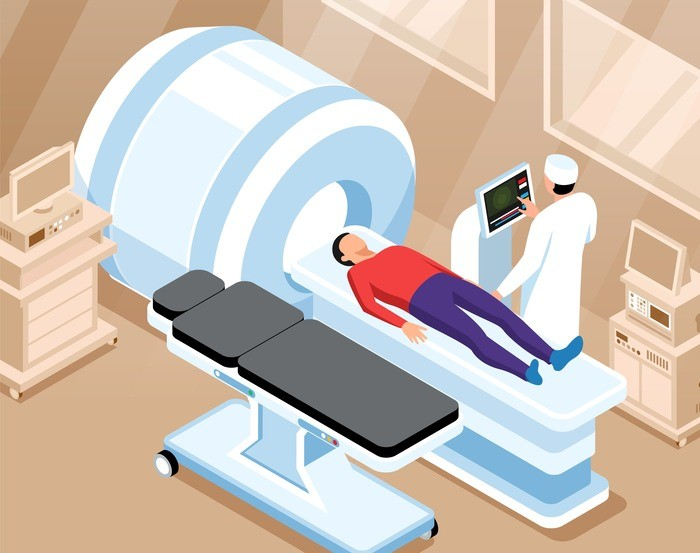
\includegraphics[width=5cm]{../images/fmri_1.jpeg}
			\caption{фМРТ сканер.} 
			\label{fg:1}
		\end{figure}		
	\end{frame}

	\begin{frame} 
		\frametitle{фМРТ}
		\begin{figure}
			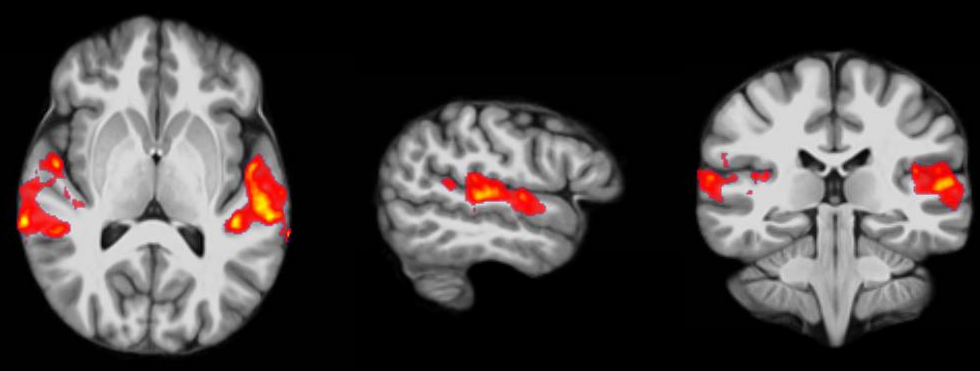
\includegraphics[width=10cm]{../images/fmri_2.png}
			\caption{МРТ скан.} 
			\label{fg:2}
		\end{figure}
	\end{frame}

	\begin{frame} 
		\frametitle{Цель работы}
		Будем считать, что мозг может функционировать в двух режимах.
		
		\begin{target_}
			Реализация и тестирование метода классификации режимов мозговой активности на основе фМРТ данных, в основе которого будут лежать синолитические сети..
		\end{target_}			
	\end{frame}

	\begin{frame} 
		\frametitle{Классификация}
		\begin{prob_task}
			Пусть есть с.в. $\xi: \Omega \rightarrow X$ и с.в. $\eta: \Omega \rightarrow Y$. Рассмотрим с.в. $(\xi, \eta): \Omega \rightarrow (X, Y)$ с распределением $p(x, y)$.
			\vspace{0.5cm}
			
			Задача классификации сводится к оценке $p(y|x)$ по выборке $(\widetilde{X}, \widetilde{Y}) = \{(x_{n}, y_{n})\}_n$.
		\end{prob_task}
	
		\begin{algo_task}
			Пусть $X$ --- множество описаний объектов, $Y$ --- множество номеров классов. Существует функция $f: X \rightarrow Y$, значения которой известны только на объектах выборки $(\widetilde{X}, \widetilde{Y}) =  \{(x_{n}, y_{n})\}_n$. 
			\vspace{0.5cm}
			
			Требуется построить алгоритм-оценку $\widehat{f}: X \rightarrow Y$.
		\end{algo_task}
	\end{frame}

	\begin{frame} 	
		\frametitle{Векторизация}	
		
		NiBabel --- библиотека предоставляющая возможность читать различные форматы файлов нейровизуализации.
		\vspace{0.5cm}
				
		\begin{figure}
			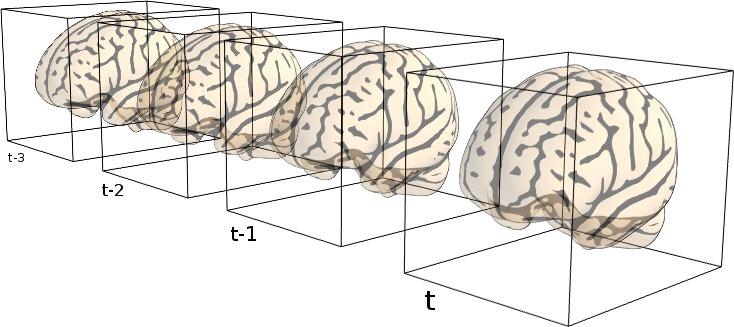
\includegraphics[width=7cm]{../images/vectorization_1.png}
			\caption{Векторизация фМРТ данных.} 
			\label{fg:5}
		\end{figure}
	\end{frame}
	
	\section{Синолитические сети}
	\begin{frame} 
		\frametitle{Основная идея (Zaikin Alexey 2022)}
		\begin{figure}
			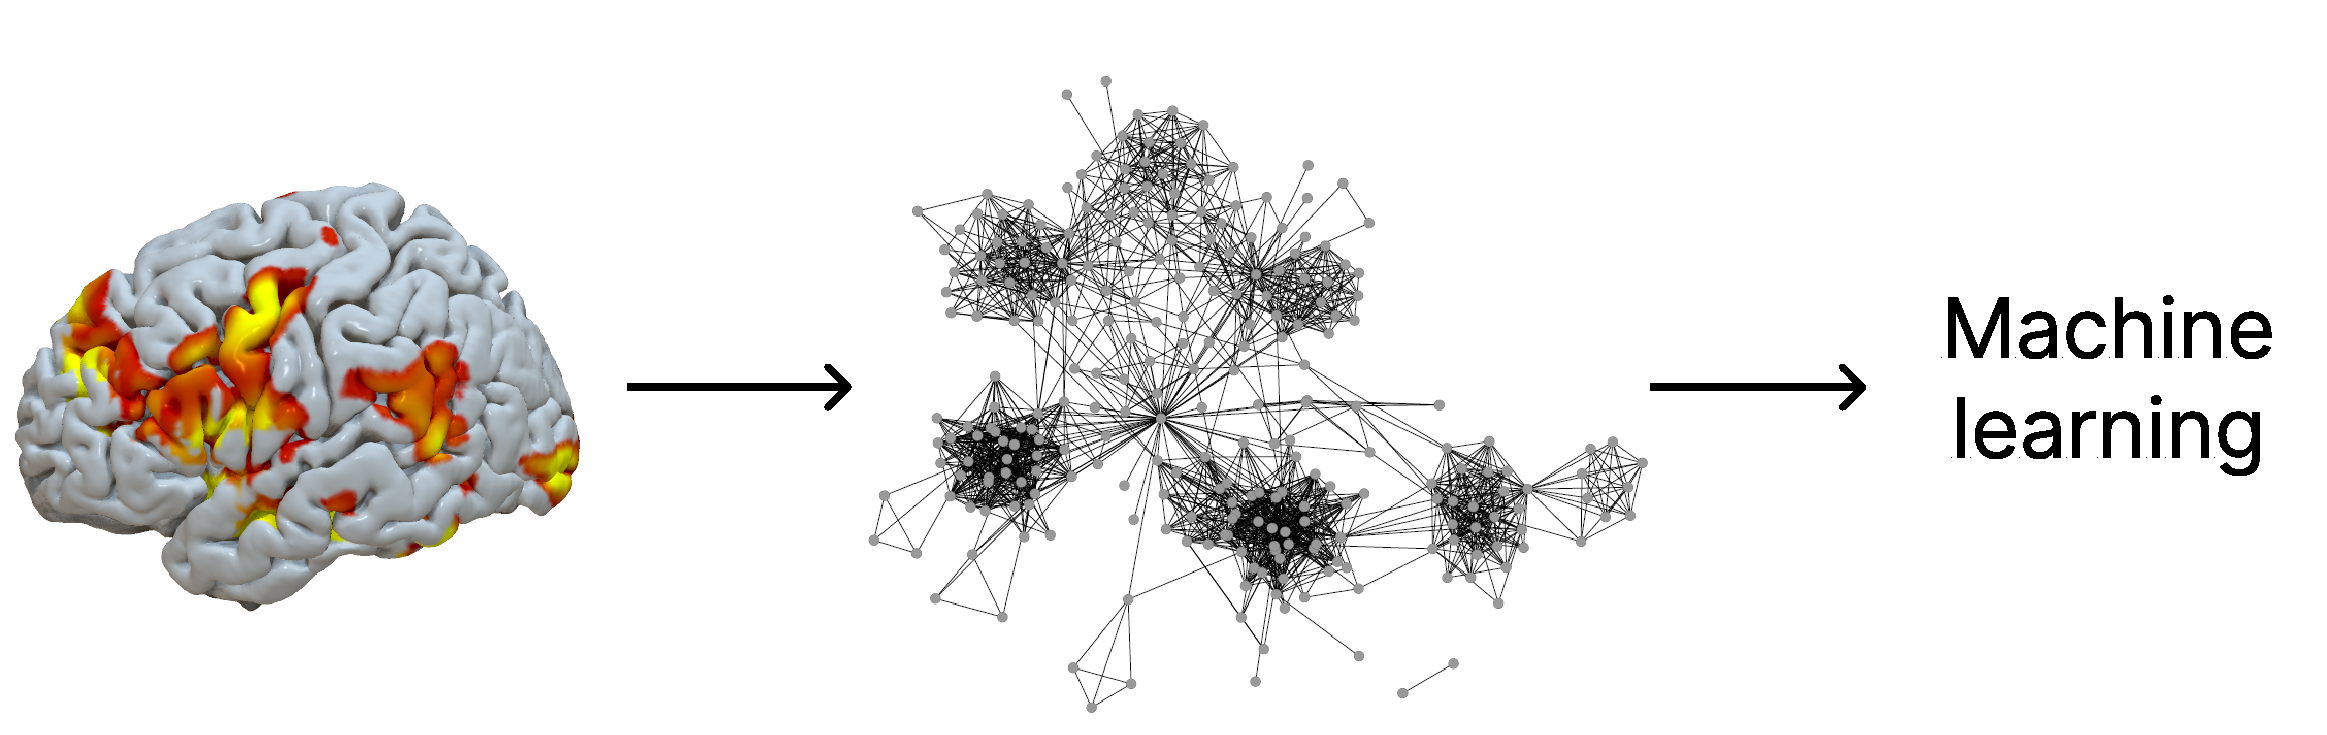
\includegraphics[width=10cm]{../images/fmri_graph_ml_1.pdf}
			\caption{Классификация на основе построения графов отражающих входные данные.} 
			\label{fg:3}
		\end{figure}
	\end{frame}

	\begin{frame} 
		\frametitle{Обозначения}
		Пусть $X$ --- множество фМРТ, а $Y = \{$\rom{1}, \rom{2}$\}$ --- режимы когнитивной активности. $(\widetilde{X}, \widetilde{Y}) =  \{(x_{n}, y_{n})\}_n$ --- конечная выборка из $(X, Y)$.
		\vspace{0.5cm}
		
		$x_k \in X$ конвертируется в массив $a^k$, на основе которого строится граф $g_k = (V_k, E_k, R_k, W_k)$, где 
		\begin{itemize}
			\item $V_k = \{v_i^k\}_i$ --- множество вершин,
			\item $E_k = \{e_{ij}^k\}_{ij}$ --- множество неориентированных ребер,
			\item $R_k = \{r_i^k\}_i$ --- множество значений вершин,
			\item $W_k = \{w_{ij}^k\}_{ij}$ --- множество весов ребер,
			\item $v_i^k$ --- вершина, отражающая область мозга $i$,
			\item $e_{ij}^k$ --- ребро, отражающее связь между областями $i$ и $j$,
			\item $r_i^k$ -- значение вершины $v_i^k$,
			\item $w_{ij}^k$ -- вес ребра $e_{ij}^k$.
		\end{itemize}									
	\end{frame}

	\begin{frame} 
		\frametitle{Подсчет весов ребер $w_{ij}^k$}						
		\begin{prob_def}
			\[
				w_{ij}^k = P(y_k = \rom{2} | r_i^k, r_j^k) - P(y_k = \rom{1} | r_i^k, r_j^k)
			\]			
		\end{prob_def}								
		Пусть $Cl_{ij}: \{y_k |(r_i^k, r_j^k), \{(r_i^n, r_j^n)\}_n, \{y_n\}_n\}_k \rightarrow [0, 1]$ --- вероятностный классификатор.
		
		\begin{algo_def}			
			\begin{equation*}
				\begin{multlined}
					w_{ij}^k = Cl_{ij}(y_k = \rom{2} | (r_i^k, r_j^k), \{(r_i^n, r_j^n)\}_n, \{y_n\}_n) - \\ - Cl_{ij}(y_k = \rom{1} | (r_i^k, r_j^k), \{(r_i^n, r_j^n)\}_n, \{y_n\}_n)
				\end{multlined}
			\end{equation*}			
		\end{algo_def}	
	\end{frame}

	\begin{frame} 
		\vspace{0.4cm}
		
		\begin{figure}
			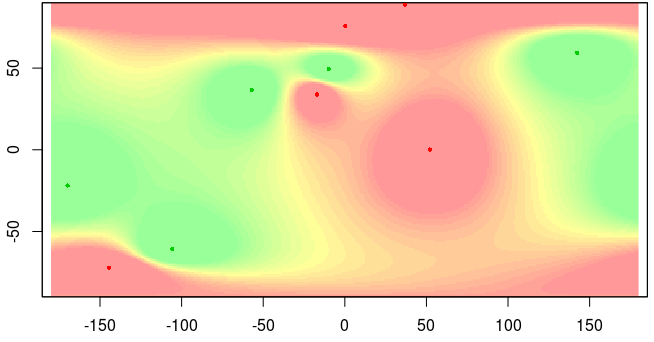
\includegraphics[width=10cm]{../images/classification.png}
			\caption{Эмпирическая плотность распределения $(r_i, r_j)$ для двух режимов, вычисленная по $\{(r_i^n, r_j^n)\}_n$.}
			\label{fg:4}
		\end{figure}
	\end{frame}	

	\section{Понижение размерности}
	\begin{frame} 
		\frametitle{Увеличение размеров вокселя}
		
		Увеличение размера шага решетки фМРТ в $n$ раз уменьшает число вокселей в $n^3$ раза.
		\vspace{0.5cm}
										
			\begin{figure}
				\begin{minipage}{3.5cm}
					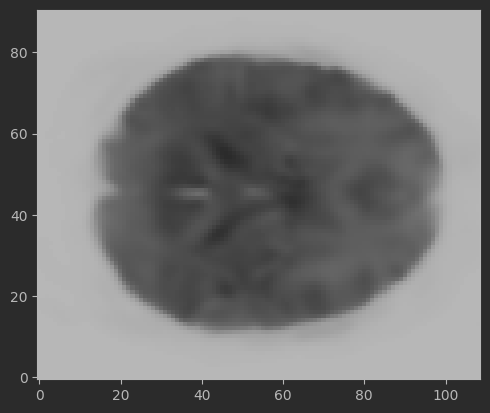
\includegraphics[width=3.5cm]{../images/downsampling2mm_1.png}
					\caption{Воксель 2 мм$^3$}
					\label{fg:6}
				\end{minipage}\hfill
				\begin{minipage}{3.5cm}
					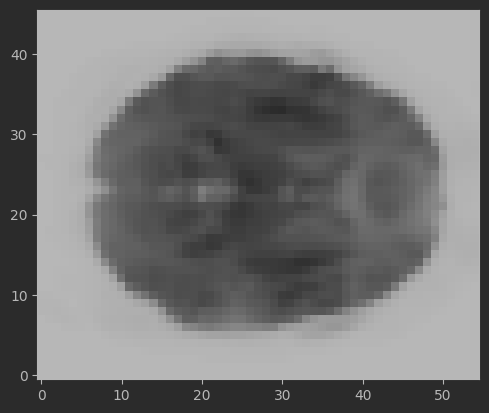
\includegraphics[width=3.5cm]{../images/downsampling4mm_2.png}
					\caption{Воксель 4 мм$^3$}
					\label{fg:7}
				\end{minipage}\hfill
				\begin{minipage}{3.5cm}
					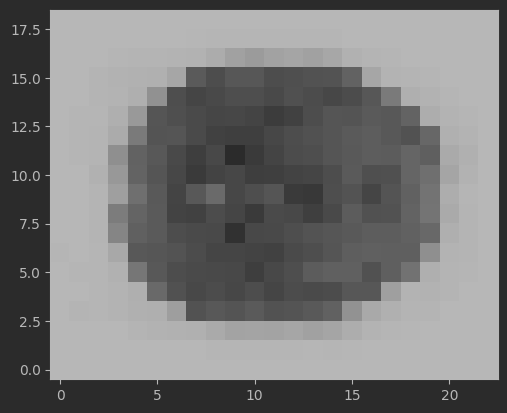
\includegraphics[width=3.5cm]{../images/downsampling10mm_3.png}
					\caption{Воксель 10 мм$^3$}
					\label{fg:8}
				\end{minipage}
			\end{figure}	
	\end{frame}
	
	\begin{frame} 
		\frametitle{Понижение размерности по времени}
		Пусть $T$ --- некоторая статистика,
		\[
		a^{kT} = T(a^k),
		\]
		т.е. для $\forall x, y, z$
		\[
		a^{kT}_{xyz} = T(\{a_{xyzt}^k : \forall t\}).
		\]
		
		\begin{figure}
			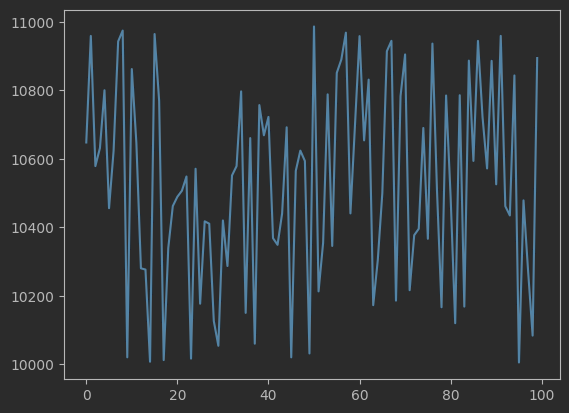
\includegraphics[width=6cm]{../images/time_series.png}
			\caption{Значения вокселя.} 
			\label{fg:11}
		\end{figure}	
	\end{frame}	

	\begin{frame} 
		\frametitle{Смена структуры графа}
		
		Построение вместо полного графа графа-сетки снижает время вычисления и требуемую память с $O(n^2)$ до $O(n)$, где $n$~--- число вершин графа.
		
		\vspace{0.5cm}
						
		\begin{figure}
			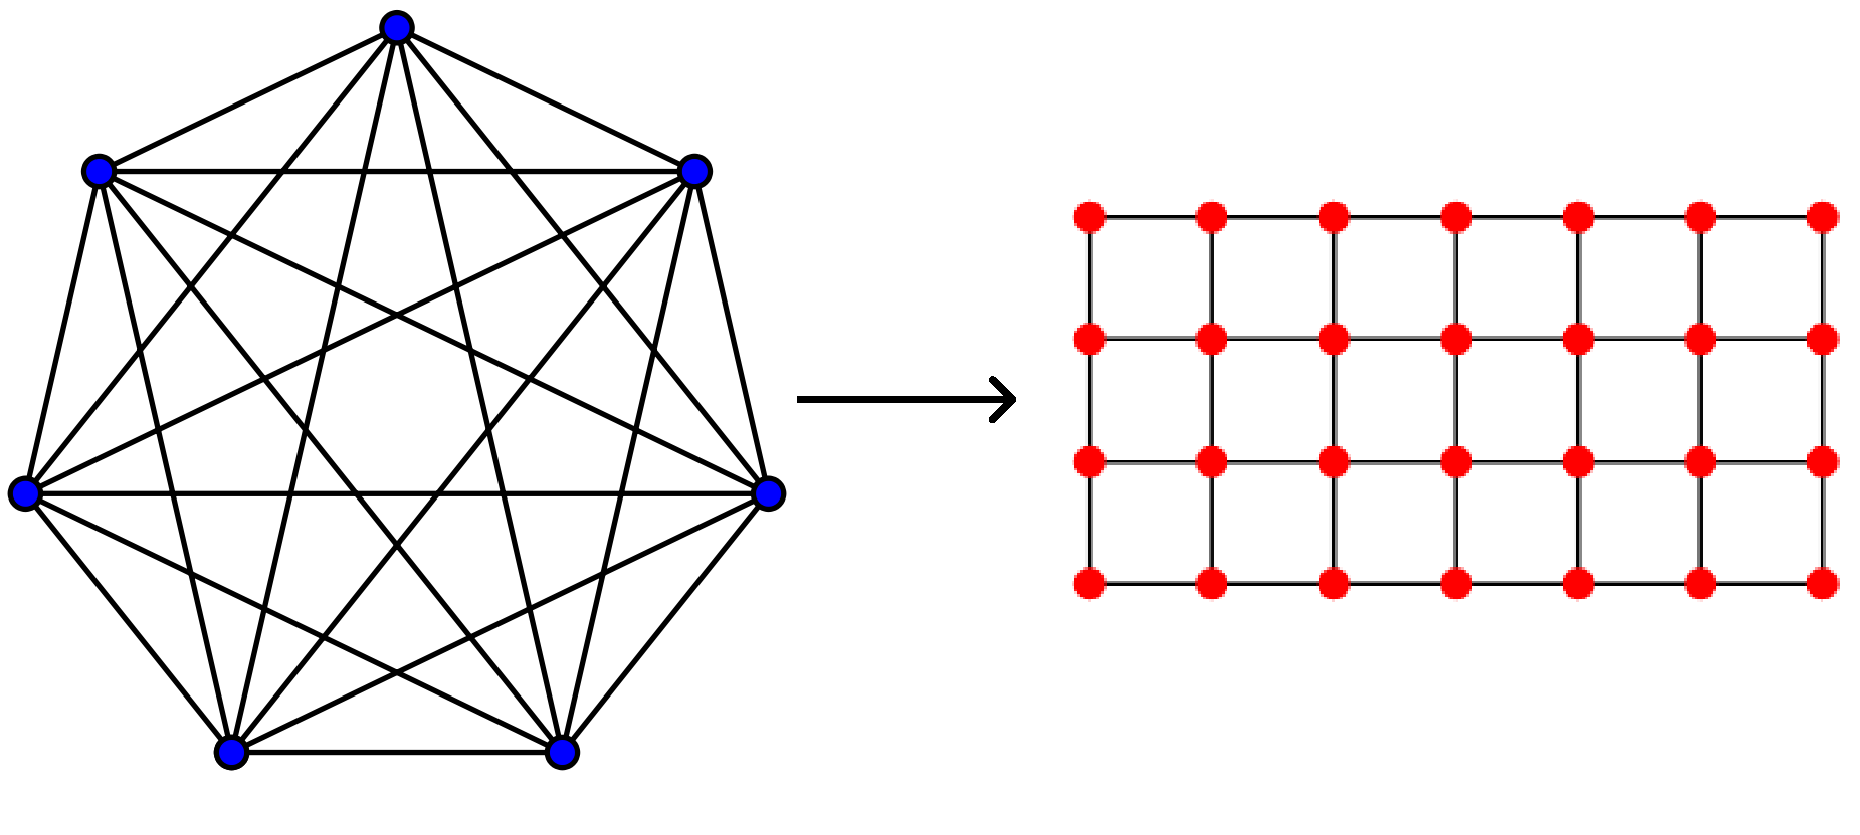
\includegraphics[width=8cm]{../images/full_grid_graphs_1.pdf}
			\caption{Смена структуры графа.} 
			\label{fg:9}
		\end{figure}			
	\end{frame}	

	\section{Алгоритм}
	\begin{frame} 
		\frametitle{Обучение модели}
		Входные данные:
		\begin{itemize}
			\item выборка $(\widetilde{X}, \widetilde{Y})$,
			\item новый размер шага решетки фМРТ $s$,
			\item статистики вокселей $\{T_m\}_m$,
			\item минимальное значение вершины $r$, для которого инцидентные с ним ребра не удаляются из графа,
			\item минимальное абсолютное значение ребра $w$, для которого ребро не удаляется из графа,
			\item характеристики графов $\{F_u\}_u$, на которых будет учиться модель.
		\end{itemize}
	\end{frame}

	\begin{frame} 
		\frametitle{Обучение модели}
		Алгоритм: 
		\begin{enumerate}
			\item изменение шага решетки фМРТ на $s$ для $\forall x_n \in \widetilde{X}$;
			\item построение $\{a^n\}_n$;
			\item вычисление $\{\{a^{nT_m}\}_{m}\}_n$;
			\item обучение  $\{Cl_{ij}\}_{ij}$ на выборке $(\{\{a^{nT_m}\}_{m}\}_n, \widetilde{Y})$;
			\item подсчет $\{W_n\}_n = \{\{w_{ij}^n\}_{ij}\}_n$ с помощью $\{Cl_{ij}\}_{ij}$ и $\{\{a^{nT_m}\}_{m}\}_n$;
			\item построение графов $\{g_n\}_n$;
			\item удаление ребер $\{e_{ij}^n : r_i^n < r | r_j^n < r | w_{ij}^n < w\}_{ij}$  для $\forall g_n$;
			\item вычисление $\{\{f^n_u\}_u\}_n = \{\{F_u(g_n)\}_u\}_n$;
			\item обучение $Cl$ на выборке $\{\{f^n_u\}_u\}_n$.
		\end{enumerate}
	\end{frame}

	\begin{frame} 
		\frametitle{Классификация}
		Входные данные:
		\begin{itemize}
			\item фМРТ $x_k$.
		\end{itemize}
		Алгоритм: 
		\begin{enumerate}
			\item изменение шага фМРТ $x_k$ решетки на $s$;
			\item построение $a^k$;
			\item вычисление $\{a^{kT_m}\}_{m}$;
			\item подсчет $W_k = \{w^k_{ij}\}_{ij}$ с помощью $\{Cl_{ij}\}_{ij}$ и $\{a^{kT_m}\}_{m}$;
			\item построение графа $g_k$;
			\item удаление из $g_k$ ребер $\{e^k_{ij} : r^k_i < r | r^k_j < r | w^k_{ij} < w\}_{ij}$;
			\item вычисление $\{f^k_u\}_u = \{F_u(g)\}_u$;
			\item классификация $\{f^k_u\}_u$ с помощью $Cl$.
		\end{enumerate}
	\end{frame}
	
	\section{Результаты}
	\begin{frame} 
		\frametitle{Данные}
		\begin{figure}
			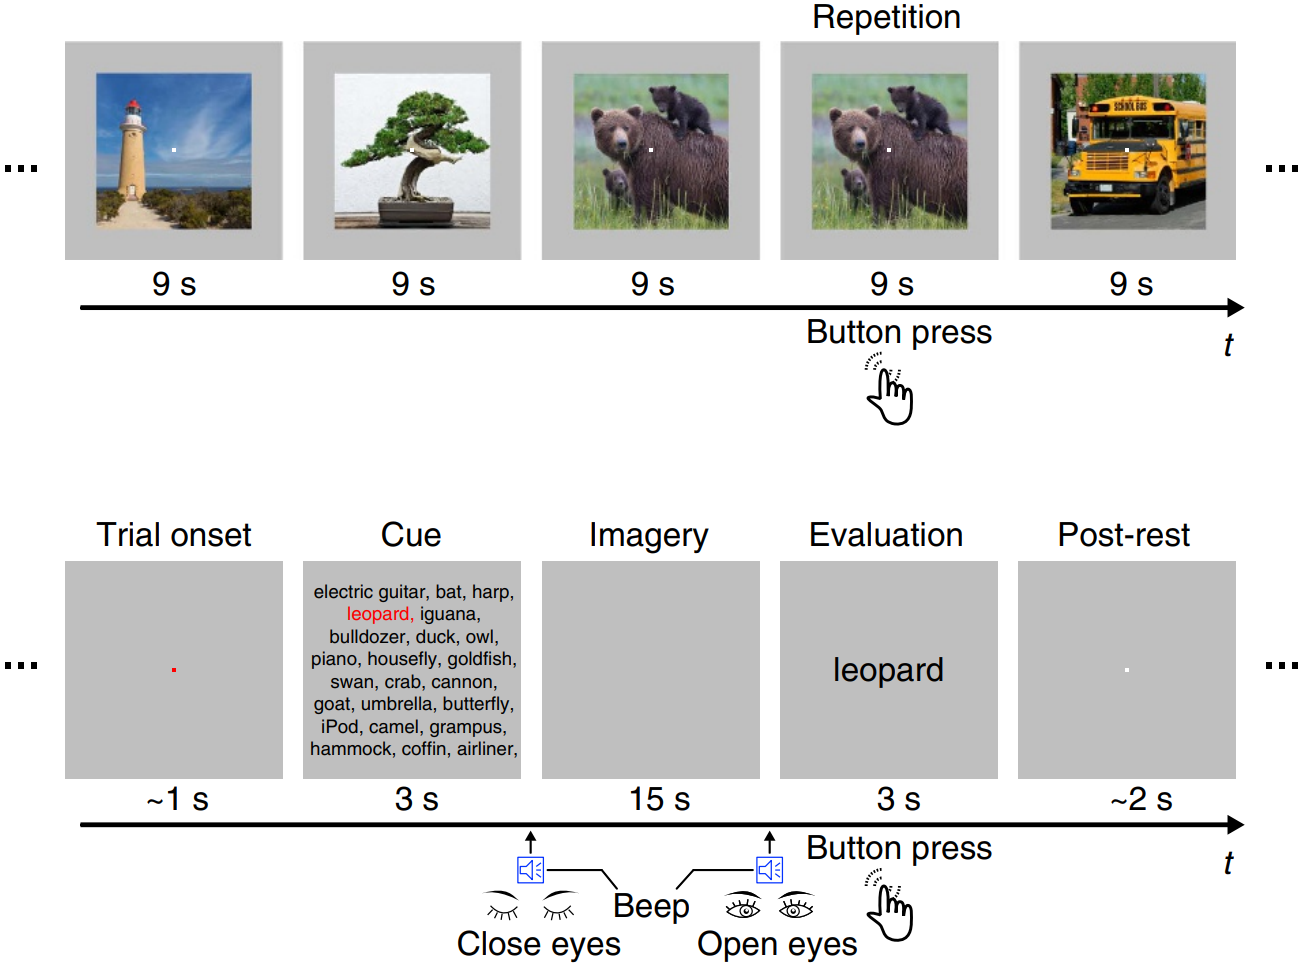
\includegraphics[width=9cm]{../images/data_3.png}
			\caption{Наблюдение или воображение объекта.} 
			\label{fg:12}
		\end{figure}
	\end{frame}

	\begin{frame} 
		\frametitle{Данные}
		\vspace{0.5cm}
		
		\begin{table}[]
			\begin{tabular}{c|cc|cc|c}
				& \multicolumn{2}{c|}{seen}            & \multicolumn{2}{c|}{imagined}        &                      \\ \cline{2-5}
				& \multicolumn{1}{c|}{training} & test & \multicolumn{1}{c|}{training} & test &                      \\ \hline
				sub-01 & \multicolumn{1}{c|}{17}       & 7    & \multicolumn{1}{c|}{14}       & 6    & 44                   \\
				sub-02 & \multicolumn{1}{c|}{17}       & 7    & \multicolumn{1}{c|}{14}       & 6    & 44                   \\
				sub-03 & \multicolumn{1}{c|}{17}       & 7    & \multicolumn{1}{c|}{14}       & 6    & 44                   \\
				sub-04 & \multicolumn{1}{c|}{17}       & 7    & \multicolumn{1}{c|}{14}       & 6    & 44                   \\
				sub-05 & \multicolumn{1}{c|}{16}       & 8    & \multicolumn{1}{c|}{14}       & 6    & 44                   \\ \hline
				& \multicolumn{1}{c|}{84}       & 36   & \multicolumn{1}{c|}{70}       & 30   & \multirow{2}{*}{220} \\ \cline{2-5}
				& \multicolumn{2}{c|}{120}             & \multicolumn{2}{c|}{100}             &                     
			\end{tabular}
			
			\caption{Разделение выборки.} 
		\end{table}
	\end{frame}

	\begin{frame} 
		\frametitle{Характеристики графов}
		\vspace{-0.75cm}
		\begin{figure}
			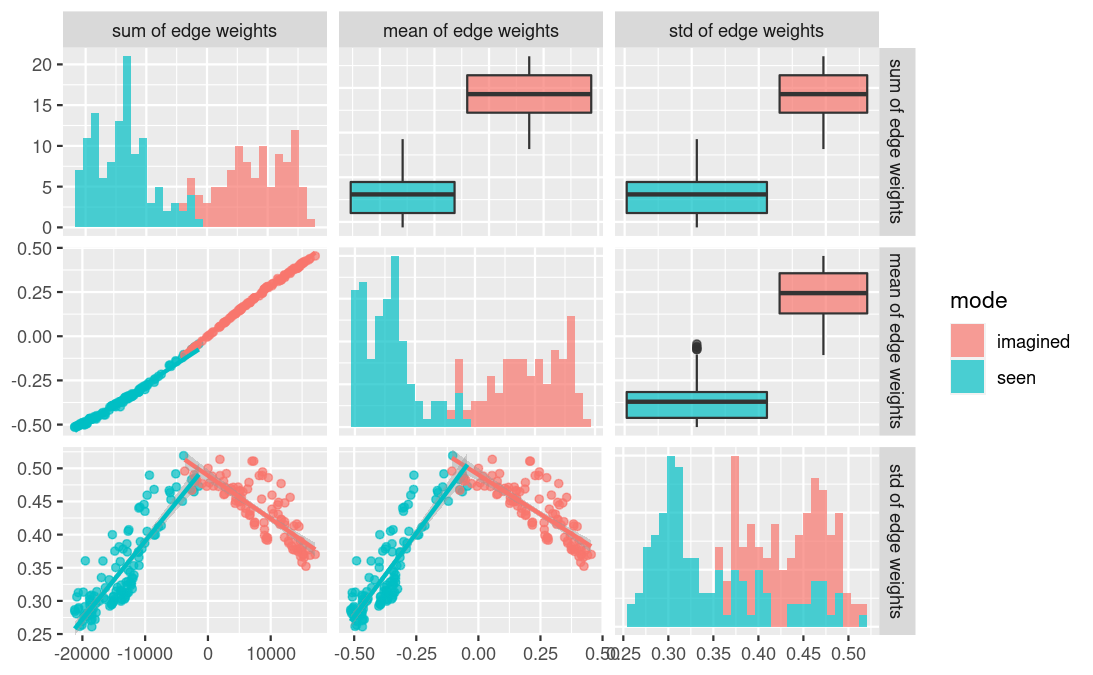
\includegraphics[width=11cm]{../images/graph_feachers_1.png}
			\caption{Распределения некоторых характеристик графов при $\{T_i\}_i = T_1$, где $T_1$ --- среднее значение вокселя.} 
			\label{fg:13}
		\end{figure}
	\end{frame}

	\begin{frame} 
		\frametitle{Характеристики графов}
		\vspace{-0.75cm}
		\begin{figure}
			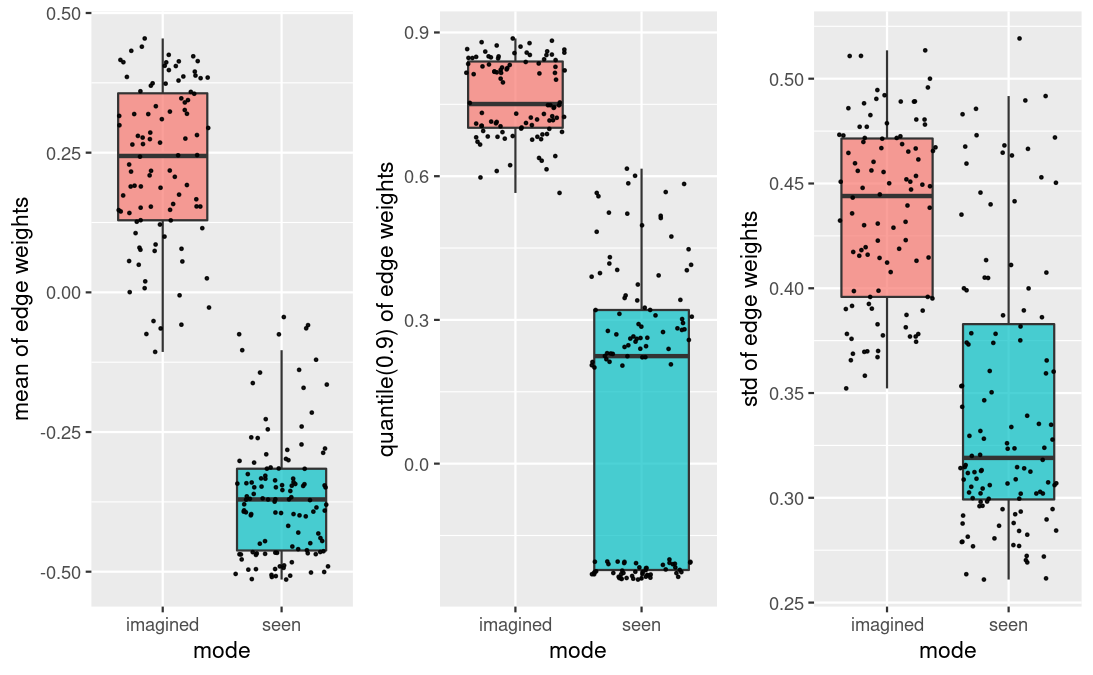
\includegraphics[width=11cm]{../images/graph_feachers_2.png}
			\caption{Распределения некоторых характеристик графов при $\{T_i\}_i = T_1$, где $T_1$ --- среднее значение вокселя.} 
			\label{fg:13}
		\end{figure}
	\end{frame}
	
	\begin{frame} 
		\frametitle{Матрицы классификации}
		\vspace{0.5cm}	

		\begin{table}
			\begin{minipage}{.5\linewidth}				
				\begin{tabular}{c|cc}
					& \multicolumn{1}{c|}{seen} & imagined \\ \hline
					seen     & 32                        & 4        \\ \cline{1-1}
					imagined & 0                         & 30      
				\end{tabular}
				\caption{$\{T_m\}_m = T_1 = mean$, точность $93.9\%$.}
			\end{minipage}%
			\begin{minipage}{.5\linewidth}				
				\begin{tabular}{c|cc}
					& \multicolumn{1}{c|}{seen} & imagined \\ \hline
					seen     & 32                        & 4        \\ \cline{1-1}
					imagined & 1                         & 29      
				\end{tabular}
				\caption{$\{T_m\}_m = T_1 = min$, точность $90.9\%$.}
			\end{minipage} 
		\end{table}
	
		\begin{table}[]
			\begin{tabular}{c|cc}
				& \multicolumn{1}{c|}{seen} & imagined \\ \hline
				seen     & 34                        & 2        \\ \cline{1-1}
				imagined & 1                         & 29      
			\end{tabular}
			\caption{$\{T_m\}_m = T_1 = quantile(0.9) - quantile(0.1)$, точность $95.5\%$.}
		\end{table}
	\end{frame}
		
		


\end{document}
	